\chapter{Supplementary deployment experiments}
\label{app:adc_replay_appendix}

This appendix collects supplementary deployment-oriented analyses that support the
main-body results of Section~\ref{sec:adc_finetuning_results} and
Section~\ref{sec:ros_pipeline_results}. The main chapter presents the most
compact figures under page constraints, while the appendix retains additional
deployment behavior that was informative during interpretation.

\section{Unfiltered single-button detector comparison}

Table~\ref{tab:appendix_unfiltered_single_button} shows the same controlled R29
single-button experiment before the baseline-model detections above 1.5~m were
removed. It is included to document the full deployment behavior of both models.
The apparent long-range advantage of the baseline model in the unfiltered distance
statistics should not be interpreted as better valid detection range, because manual
review showed that all twelve baseline detections above 1.5~m were false positives.

\begin{table}[htbp]
    \centering
    \caption{Unfiltered controlled single-button comparison on the same recorded \gls{ros} bag from HAN Building R29.}
    \label{tab:appendix_unfiltered_single_button}
    \small
    \begin{tabular}{lcc}
        \toprule
        Metric & Baseline model & \glsentryshort{adc} fine-tuned model \\
        \midrule
        Frames with detected buttons & 116 & 138 \\
        Mean target confidence & 0.7855 & 0.8069 \\
        Median target confidence & 0.8328 & 0.8423 \\
        Mean valid-target distance [m] & 0.4408 & 0.4282 \\
        Median valid-target distance [m] & 0.3353 & 0.4102 \\
        Maximum valid-target distance [m] & 1.6536 & 0.8761 \\
        \bottomrule
    \end{tabular}
\end{table}

\section{Single-button end-to-end confidence behavior}

Besides the detector-only baseline-versus-\glsentryshort{adc} comparison shown in the main
body, the controlled single-button R29 replay was also inspected at the full
\gls{yolo}+\gls{ocr} pipeline level. Figure~\ref{fig:appendix_single_button_yolo_ocr_confidence}
shows the detector confidence together with the downstream \gls{ocr} confidence
for the same run. Correct \texttt{UP} reads remain clustered in the lower-to-mid
distance range, while the few \gls{ocr} errors appear at larger distances within
that run.

\begin{figure}[htbp]
    \centering
    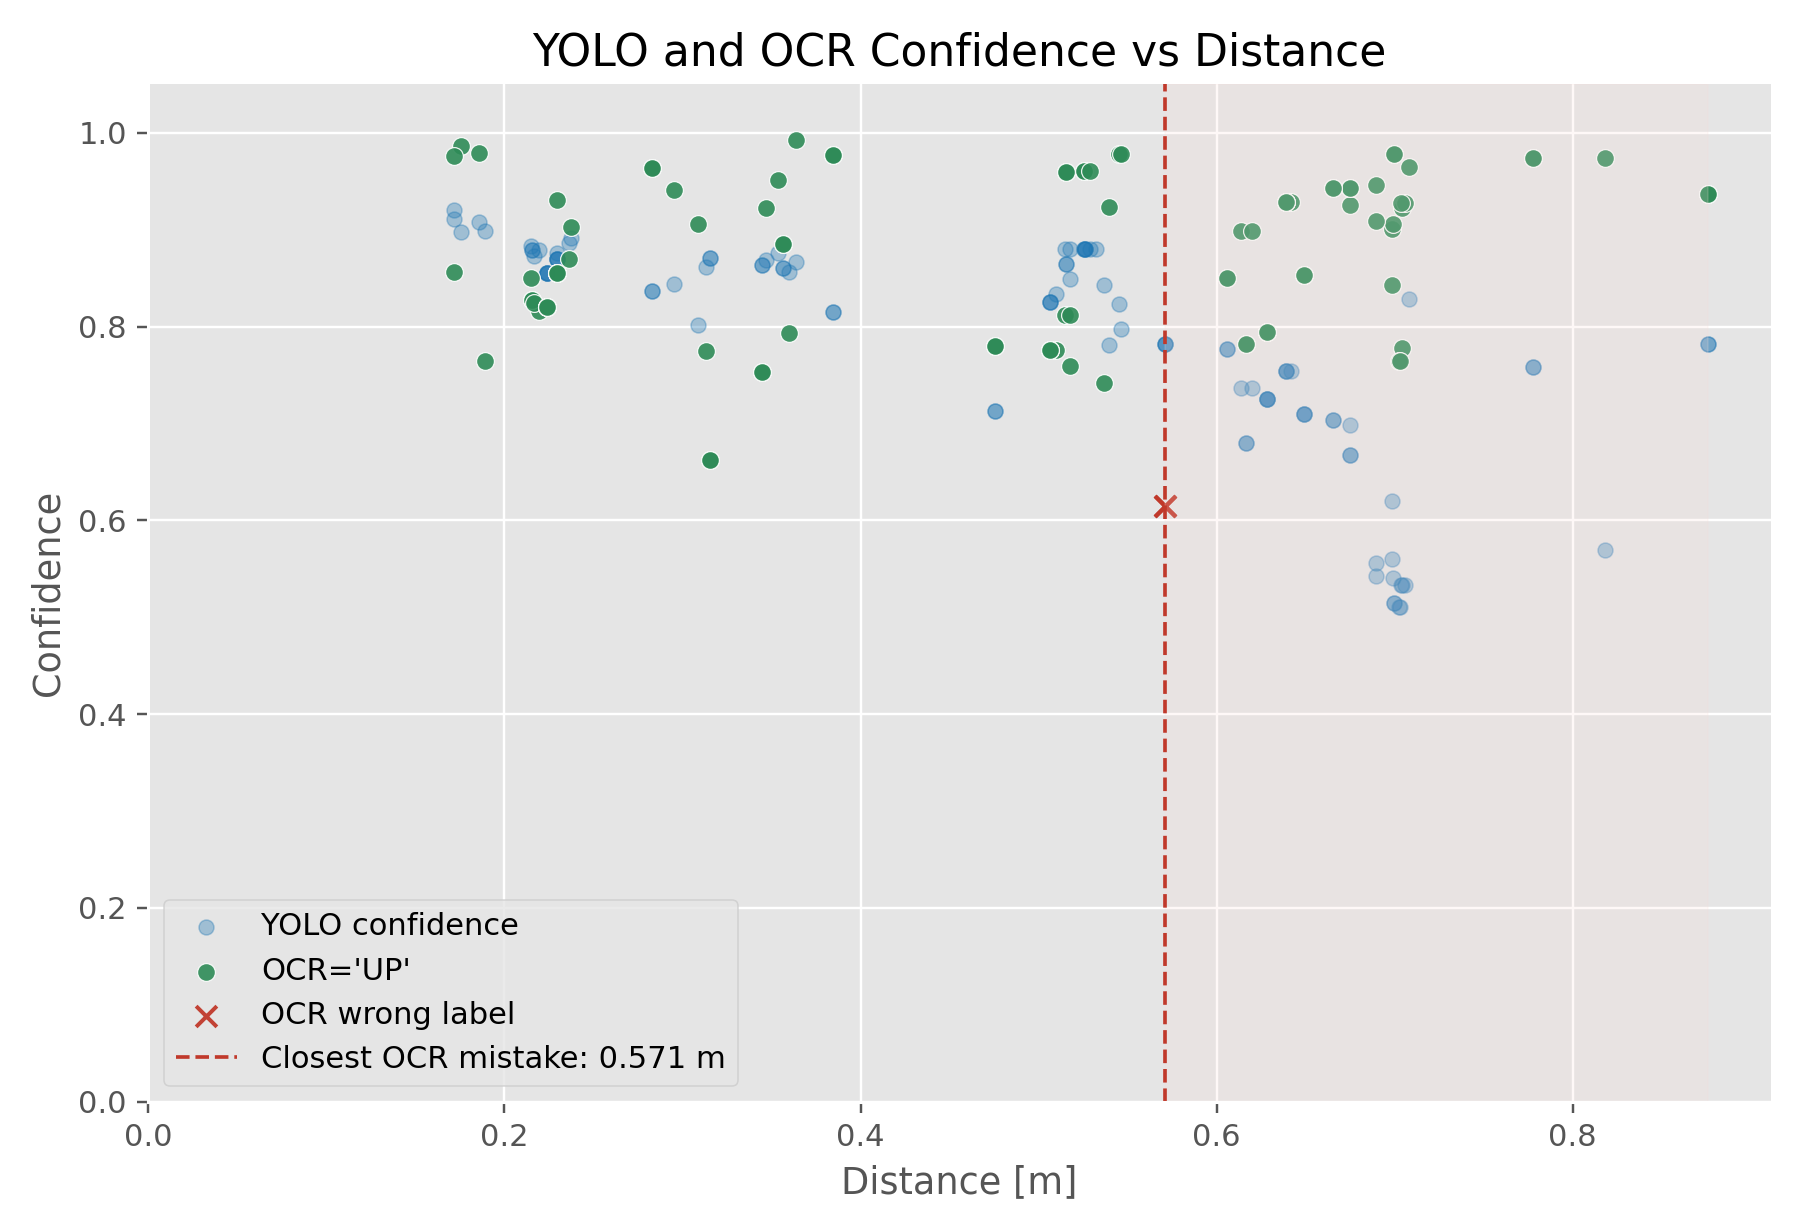
\includegraphics[width=0.82\textwidth]{figures/appendices/single_button_yolo_ocr_confidence_distance.png}
    \caption{Supplementary single-button R29 replay plot showing \gls{yolo} confidence, \gls{ocr} confidence, and the distances at which \gls{ocr} stopped reading the \texttt{UP} button correctly.}
    \label{fig:appendix_single_button_yolo_ocr_confidence}
\end{figure}

\section{Mixed-environment replay review by distance bin}

A second replay analysis was performed on a longer university elevator bag that
contained multiple panels, cluttered backgrounds, and changing viewpoints. The
detections were manually reviewed as true positives or false positives after
replay. Figure~\ref{fig:appendix_reviewed_tp_fp_distance_bins} shows the reviewed
true- and false-positive counts by distance bin for that broader run. The figure
is included as supporting evidence for the realistic deployment trend discussed
in Section~\ref{sec:ros_pipeline_results}: reviewed detections were highly
reliable below roughly 1.5~m, whereas the longer-range bins were dominated by
false positives.

\begin{figure}[htbp]
    \centering
    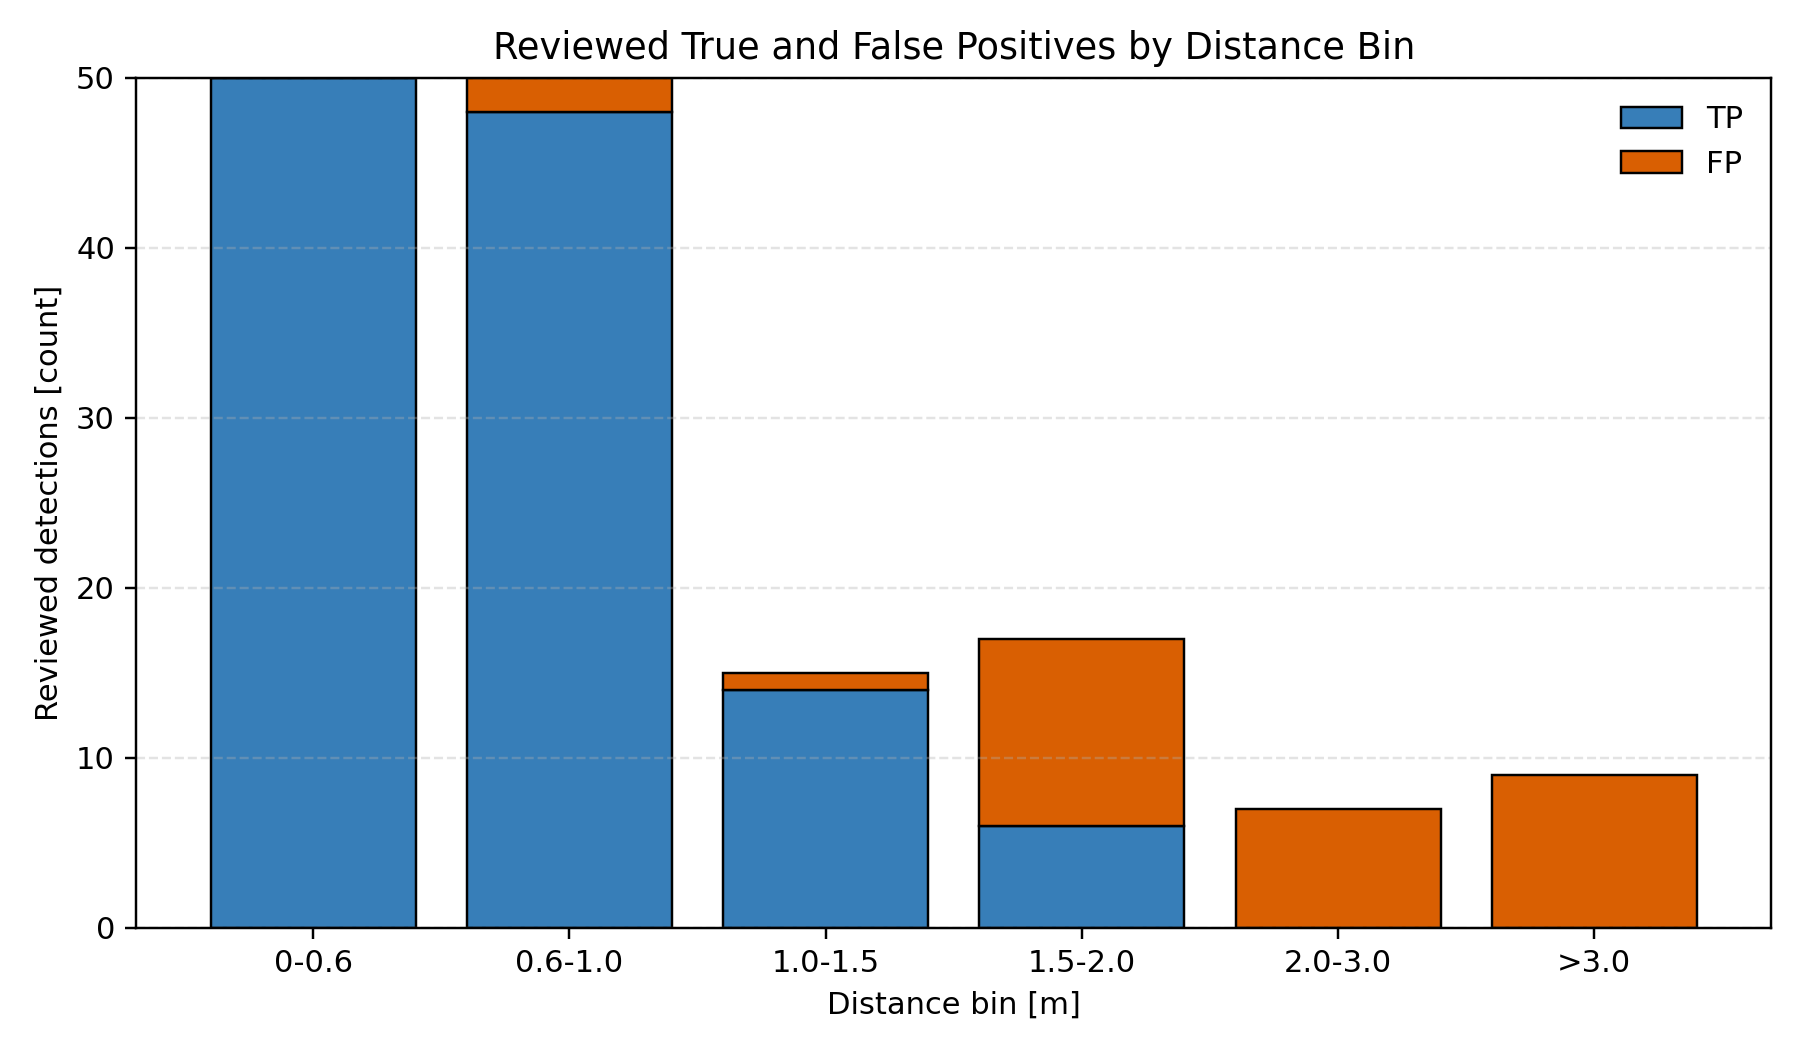
\includegraphics[width=0.82\textwidth]{figures/appendices/reviewed_tp_fp_by_distance_bin.png}
    \caption{Reviewed true and false positive detections by distance bin on the longer university replay run. Close-range bins were sampled, while the longer-distance bins were reviewed exhaustively.}
    \label{fig:appendix_reviewed_tp_fp_distance_bins}
\end{figure}
